% BHU PYQ -- Professional Exam Template
\documentclass[11pt,a4paper]{article}

\usepackage[a4paper,top=2.5cm,bottom=2.5cm,left=2.8cm,right=2.8cm,headheight=14pt]{geometry}
\usepackage{amsmath,amssymb}
\usepackage[T1]{fontenc}
\usepackage[utf8]{inputenc}
\usepackage{lmodern}
\usepackage{microtype}
\usepackage{fancyhdr}
\usepackage{enumitem}
\usepackage{hyperref}
\usepackage{lastpage}
\usepackage{parskip}
\usepackage{tikz}
\usetikzlibrary{arrows.meta,shapes,positioning}

\hypersetup{colorlinks=true,urlcolor=black,linkcolor=black,
  pdftitle={B.Sc. (Hons.) Zoology Sem-V ZOB-504 -- BHU PYQ}}

\pagestyle{fancy}
\fancyhf{}
\renewcommand{\headrulewidth}{0.4pt}
\renewcommand{\footrulewidth}{0.4pt}
\fancyhead[L]{\small   \textit{Banaras Hindu University}}
\fancyhead[R]{\small   \textit{Zoology Paper: ZOB-504}}
\fancyfoot[C]{\small Page  \thepage\ of \pageref{LastPage}}


\newlist{parts}{enumerate}{3}
\setlist[parts,1]{label=(\alph*),leftmargin=*,itemsep=4pt,topsep=3pt}
\setlist[parts,2]{label=(\roman*),leftmargin=*,itemsep=2pt,topsep=2pt}
\setlist[parts,3]{label=(\arabic*),leftmargin=*,itemsep=2pt,topsep=2pt}

\newcommand{\pts}[1]{\hfill   \textit{[#1]}}


\begin{document}


\begin{center}
  {\large\bfseries BANARAS HINDU UNIVERSITY}\\[2pt]
  {
\normalsize B.Sc. (Hons.) Semester V Examination, 2022-23}\\[6pt]
  \rule{0.8\linewidth}{0.5pt}\\[6pt]
  {\large\bfseries Zoology}\\[4pt]
  {\large\bfseries Paper: ZOB-504 --- Biotechniques}\\[4pt]
  {
\normalsize Time: Three hours \hfill Full Marks: 70}
\end{center}

\rule{\linewidth}{0.4pt}

\smallskip



\noindent   \textit{Note: Answer six questions including Question No. 1 which is compulsory. The figures in the right-hand margin indicate marks.}

\bigskip




\noindent   \textbf{Question 1.} Answer the following parts:

\begin{parts}
  \item Select and write the best options in the following:\pts{$4  \times 0.5 = 2$}
  
\begin{parts}
    \item In gel electrophoresis, the detergent sodium dodecyl is used to:
    
\begin{parts}
      \item adjust the pH of protein
      \item renature protein
      \item make the protein positively charged
      \item make the protein negatively charged
    \end{parts}
    
    \item Which is the stain commonly used in electron microscopy?
    
\begin{parts}
      \item Uranyl acetate
      \item Lead citrate
      \item Both (a) and (b)
      \item None of the above
    \end{parts}

    \item The pH indicator in animal cell culture medium is:
    
\begin{parts}
      \item methyl red
      \item phenol red
      \item methyl orange
      \item All of the above
    \end{parts}

    \item Formalin solution (10\% unbuffered) is composed of:
    
\begin{parts}
      \item 10 ml formaldehyde (40\%) and 90 ml distilled water
      \item 50 ml formaldehyde (40\%) and 50 ml distilled water
      \item 10 ml formaldehyde (10\%) and 90 ml distilled water
      \item 50 ml formaldehyde (10\%) and 50 ml distilled water
    \end{parts}
  \end{parts}
  
  \item State whether the following statements are True or False. Justify your answer in brief:\pts{$3  \times 2 = 6$}
  
\begin{parts}
    \item In a phase-contrast microscope, the undiffracted or background light is retarded by the phase plate.
    \item The wavelength of electrons is dependent on the accelerating voltage.
    \item Differential centrifugation is based on the difference in the size of biological particles of different densities.
  \end{parts}

  \item Define the following:\pts{$4  \times 1 = 4$}
  
\begin{parts}
    \item $ \text{R}_{ \text{f}}$ value
    \item Microtome
    \item Critical point drying
    \item Limit of resolution
  \end{parts}

  \item Expand the following:\pts{$4  \times 0.5 = 2$}
  
\begin{parts}
    \item EDTA
    \item DMEM
    \item TEMED
    \item LASER
  \end{parts}

  \item Differentiate between the following:\pts{$2  \times 3 = 6$}
  
\begin{parts}
    \item Bright field and Dark field microscope
    \item Paper and Thin layer chromatography
  \end{parts}
\end{parts}

\medskip


\noindent   \textbf{Question 2.} Write down the principle of centrifugation. Discuss the applications of analytical centrifugation.\pts{10}

\pagebreak

\medskip


\noindent   \textbf{Question 3.} What do you understand by electrophoretic mobility? Discuss the procedure of electrophoretic separation of nucleic acids.\pts{10}


\begin{center}

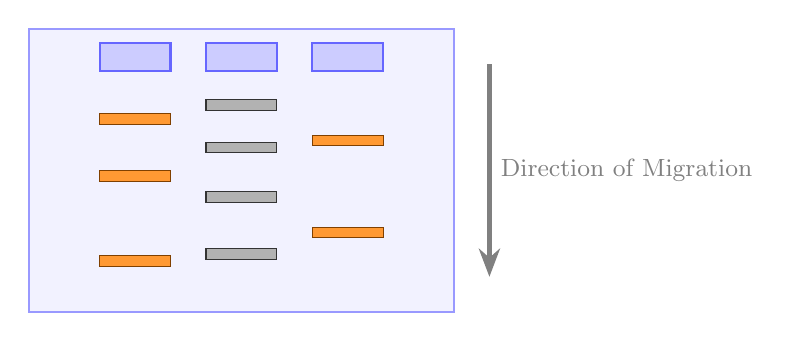
\begin{tikzpicture}[scale=0.9, >=Stealth, every node/.style={font=\small}]
  % Gel background
  \draw[fill=blue!5, draw=blue!40, thick] (0,0) rectangle (6,-4);
  
ode[right] at (6, -2) {   \textbf{Agarose Gel}};
  
  % Electrodes
  
ode[left, red!85!black] at (-0.5, -0.5) {   \textbf{-- Anode}};
  
ode[left, green!50!black] at (-0.5, -3.5) {   \textbf{+ Cathode}};
  
  % Wells
  \foreach \x in {1, 2.5, 4} {
    \draw[fill=blue!20, draw=blue!60, thick] (\x, -0.2) rectangle (\x+1, -0.6);
  }
  
ode[above] at (3, 0) {Sample Wells};
  
  % DNA Bands in lane 1
  \draw[fill=orange!80, draw=orange!50!black] (1, -1.2) rectangle (2, -1.35);
  \draw[fill=orange!80, draw=orange!50!black] (1, -2.0) rectangle (2, -2.15);
  \draw[fill=orange!80, draw=orange!50!black] (1, -3.2) rectangle (2, -3.35);
  
  % DNA Bands in lane 2 (Ladder)
  \draw[fill=gray!60, draw=gray!40!black] (2.5, -1.0) rectangle (3.5, -1.15);
  \draw[fill=gray!60, draw=gray!40!black] (2.5, -1.6) rectangle (3.5, -1.75);
  \draw[fill=gray!60, draw=gray!40!black] (2.5, -2.3) rectangle (3.5, -2.45);
  \draw[fill=gray!60, draw=gray!40!black] (2.5, -3.1) rectangle (3.5, -3.25);
  
  % DNA Bands in lane 3
  \draw[fill=orange!80, draw=orange!50!black] (4, -1.5) rectangle (5, -1.65);
  \draw[fill=orange!80, draw=orange!50!black] (4, -2.8) rectangle (5, -2.95);
  
  % Direction of migration
  \draw[->, ultra thick, gray] (6.5, -0.5) -- (6.5, -3.5) node[midway, right] {Direction of Migration};
  
  % Sizes
  
ode[left, font=\scriptsize] at (2.4, -1.07) {10 kb};
  
ode[left, font=\scriptsize] at (2.4, -1.67) {5 kb};
  
ode[left, font=\scriptsize] at (2.4, -2.37) {2 kb};
  
ode[left, font=\scriptsize] at (2.4, -3.17) {0.5 kb};
\end{tikzpicture}
\end{center}

\medskip


\noindent   \textbf{Question 4.} Answer the following:

\begin{parts}
  \item Write down the factors that affect the fixation of biological tissue samples.\pts{5}
  \item Describe briefly the hematoxylin and eosin staining methods of paraffin-embedded tissue sections.\pts{5}
\end{parts}

\medskip


\noindent   \textbf{Question 5.} Describe with a labeled diagram, the working principles and applications of the fluorescence microscope.\pts{10}


\begin{center}

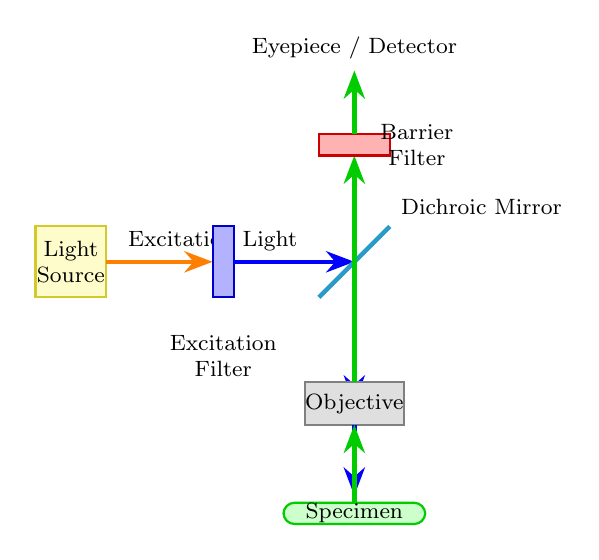
\begin{tikzpicture}[scale=0.9, >=Stealth, every node/.style={font=\footnotesize}]
  % Light source
  \draw[fill=yellow!20, draw=yellow!80!black, thick] (-4, 2) rectangle (-3, 3) node[pos=0.5, align=center] {Light\\Source};
  \draw[ultra thick, orange, ->] (-3, 2.5) -- (-1.5, 2.5) node[above, black] {Excitation Light};
  
  % Excitation filter
  \draw[fill=blue!30, draw=blue!80!black, thick] (-1.5, 2) rectangle (-1.2, 3) node[below=0.8cm, pos=0.5, align=center] {Excitation\\Filter};
  \draw[ultra thick, blue, ->] (-1.2, 2.5) -- (0.5, 2.5);
  
  % Dichroic Mirror
  \draw[ultra thick, cyan!80!black] (0, 2) -- (1, 3) node[above right, black] {Dichroic Mirror};
  
  % Excitation light reflected downwards
  \draw[ultra thick, blue, ->] (0.5, 2.5) -- (0.5, 0.5);
  
  % Objective lens
  \draw[fill=gray!25, draw=gray, thick] (-0.2, 0.2) rectangle (1.2, 0.8) node[pos=0.5] {Objective};
  \draw[ultra thick, blue, ->] (0.5, 0.2) -- (0.5, -0.8);
  
  % Specimen
  \draw[fill=green!20, draw=green!80!black, rounded corners, thick] (-0.5, -1.2) rectangle (1.5, -0.9) node[pos=0.5] {Specimen};
  
  % Emitted light
  \draw[ultra thick, green!80!black, ->] (0.5, -0.9) -- (0.5, 0.2);
  \draw[ultra thick, green!80!black, ->] (0.5, 0.8) -- (0.5, 2.5) -- (0.5, 4);
  
  % Emission/Barrier Filter
  \draw[fill=red!30, draw=red!80!black, thick] (0, 4) rectangle (1, 4.3) node[right=0.2cm, pos=0.5, align=center] {Barrier\\Filter};
  \draw[ultra thick, green!80!black, ->] (0.5, 4.3) -- (0.5, 5.2) node[above, black] {Eyepiece / Detector};
\end{tikzpicture}
\end{center}

\medskip


\noindent   \textbf{Question 6.} Define radioactivity. Explain the various methods used for the detection and measurement of radioactivity.\pts{10}

\pagebreak

\medskip


\noindent   \textbf{Question 7.} Describe different types of animal cell culture. Write down a stepwise procedure to initiate culture from animal tissues.\pts{10}

\medskip


\noindent   \textbf{Question 8.} Write short notes on the following:\pts{$2  \times 5 = 10$}

\begin{parts}
  \item Cell viability test
  \item Spectrophotometer
  
  
\begin{center}
  
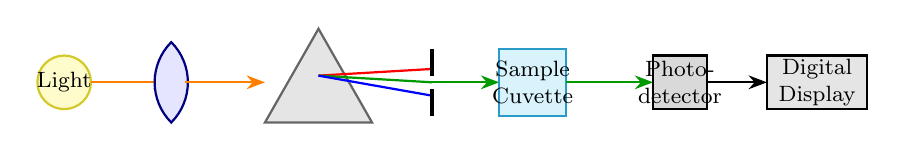
\begin{tikzpicture}[scale=0.85, >=Stealth, every node/.style={font=\footnotesize}]
    % Light source
    \draw[fill=yellow!20, draw=yellow!80!black, thick] (-5, 0) circle (0.4) node {Light};
    \draw[->, thick, orange] (-4.6, 0) -- (-3.4, 0);
    
    % Collimator Lens
    \draw[fill=blue!10, draw=blue!50!black, thick] (-3.4, -0.6) to[out=45, in=-45] (-3.4, 0.6) to[out=225, in=135] (-3.4, -0.6) -- cycle;
    
ode[below=0.7cm] at (-3.4, 0) {Lens};
    \draw[->, thick, orange] (-3.2, 0) -- (-2, 0);
    
    % Monochromator Prism
    \draw[fill=gray!20, draw=gray!80!black, thick] (-2, -0.6) -- (-1.2, 0.8) -- (-0.4, -0.6) -- cycle;
    
ode[above=0.8cm] at (-1.2, -0.6) {Prism};
    
    % Light dispersion
    \draw[thick, red] (-1.2, 0.1) -- (0.5, 0.2);
    \draw[thick, green!60!black] (-1.2, 0.1) -- (0.5, 0.0);
    \draw[thick, blue] (-1.2, 0.1) -- (0.5, -0.2);
    
    % Slit
    \draw[ultra thick, black] (0.5, 0.5) -- (0.5, 0.1);
    \draw[ultra thick, black] (0.5, -0.5) -- (0.5, -0.1);
    
ode[below=0.6cm] at (0.5, 0) {Slit};
    
    % Selected wavelength
    \draw[thick, green!60!black, ->] (0.5, 0) -- (1.5, 0);
    
    % Cuvette
    \draw[fill=cyan!15, draw=cyan!80!black, thick] (1.5, -0.5) rectangle (2.5, 0.5) node[pos=0.5, align=center] {Sample\\Cuvette};
    \draw[thick, green!60!black, ->] (2.5, 0) -- (3.8, 0);
    
    % Detector
    \draw[fill=gray!30, draw=black, thick] (3.8, -0.4) rectangle (4.6, 0.4) node[pos=0.5, align=center] {Photo-\\detector};
    \draw[->, thick] (4.6, 0) -- (5.5, 0);
    
    % Digital Display
    \draw[fill=black!10, draw=black, thick] (5.5, -0.4) rectangle (7, 0.4) node[pos=0.5, align=center] {Digital\\Display};
  \end{tikzpicture}
  \end{center}
\end{parts}

\vfill
\rule{\linewidth}{0.4pt}

\begin{center}\small
\href{https://bhu-exam.vercel.app/}{Click Here}\\[4pt]\href{https://me-aryan.vercel.app/}{Click Here}\\[4pt]\href{https://quashan-me.vercel.app/}{Click Here}
\end{center}

\end{document}
